\chapter{外文资料的调研阅读报告或书面翻译}
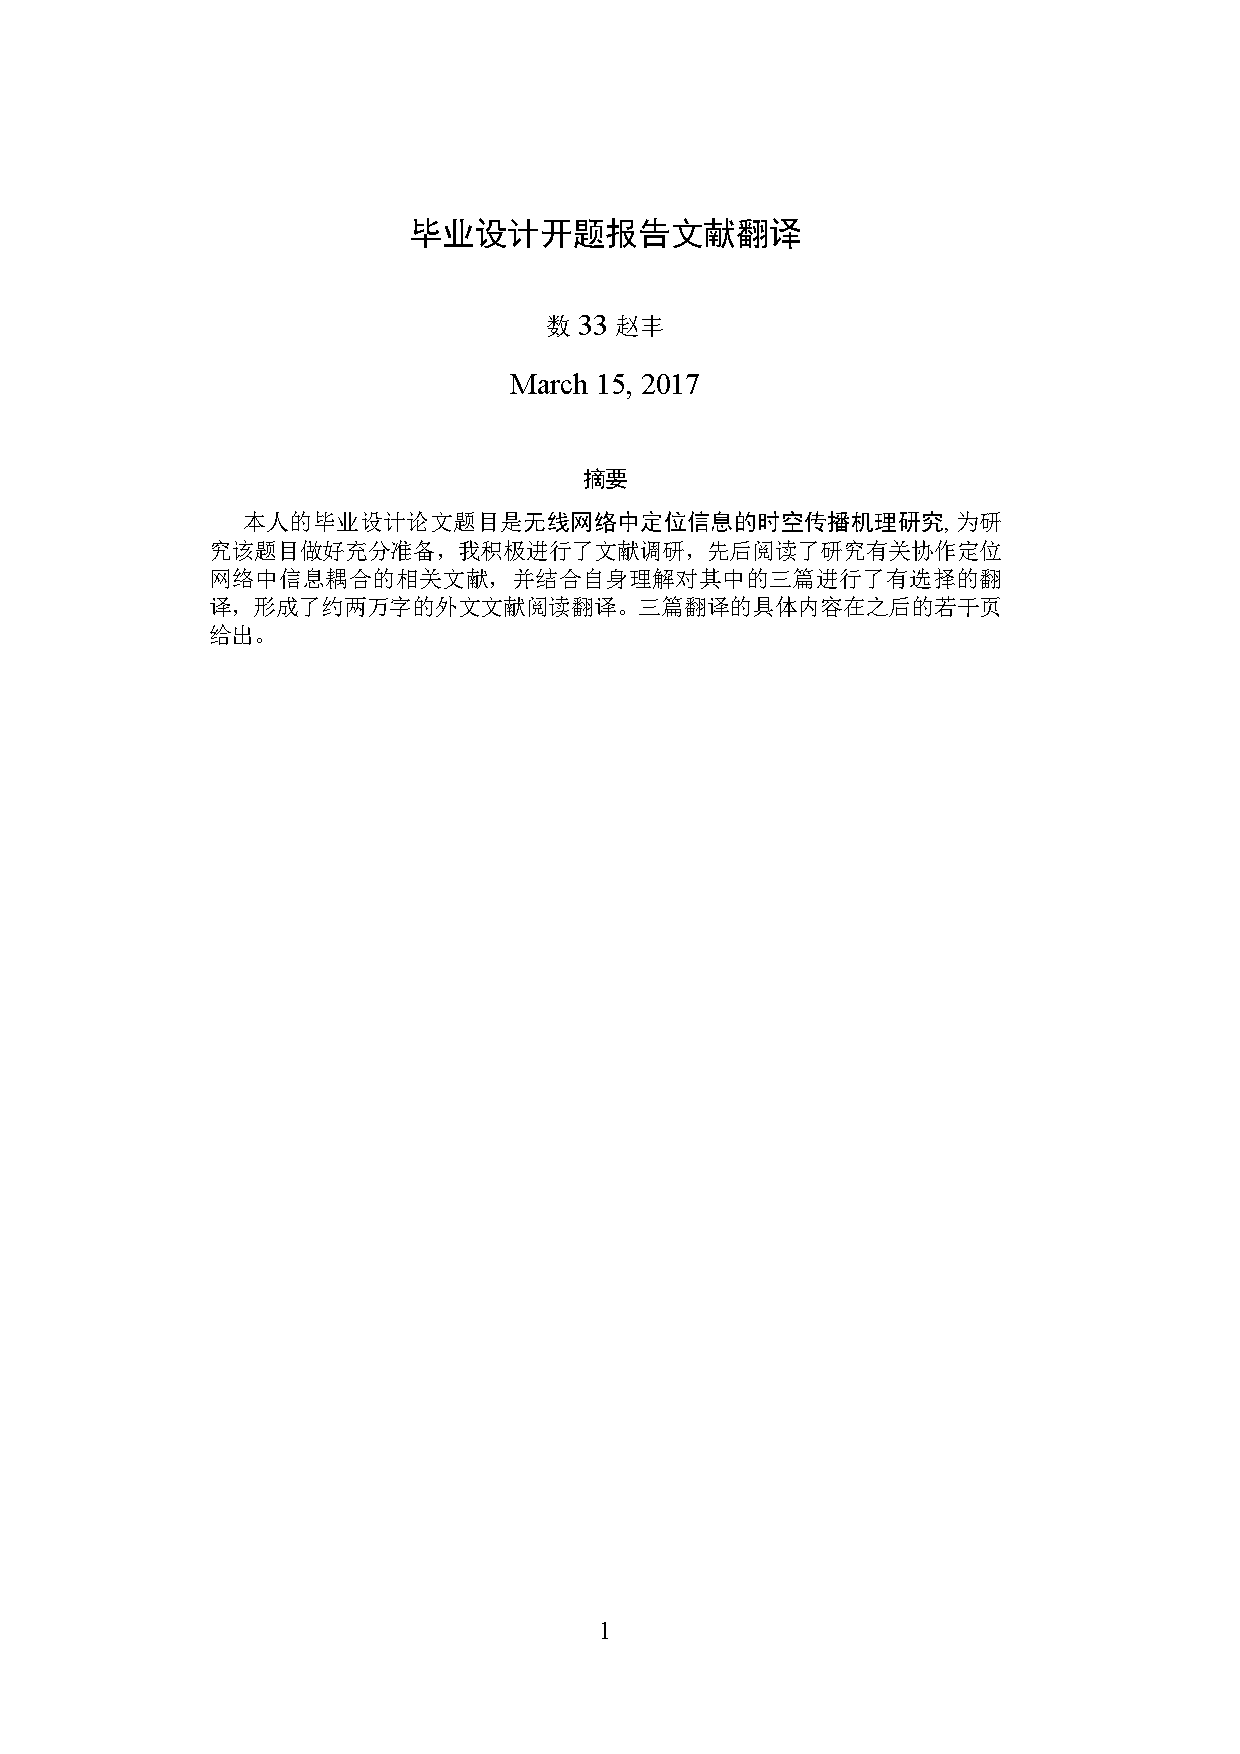
\includepdf[pages=-]{translation.pdf}
\chapter{公式的推导}
\section{建模过程的一些推导过程}
\subsection{定位问题中费舍尔信息矩阵一般结构推导}\label{A_F_1}
在非协作单节点定位中,测量量的联合概率分布由式(\ref{eq:single})给出,费舍尔信息矩阵是费舍尔信息量的自然推广,在满足一定正则性的条件下,费舍尔信息矩阵可以写成:
\begin{equation}
I(\bm{p})=-\mathbb{E}_{\bm{x}}(\bigtriangledown_{\bm{p}} \log f(\vec{x}|\bm{p}))^T(\bigtriangledown_{\bm{p}} \log f(\vec{x}|\bm{p}))
\end{equation}
其中f是随机向量$\vec{x}$的密度函数,利用上面的公式,首先对式(\ref{eq:single})取对数并求梯度得:
\begin{equation}
\bigtriangledown_{\bm{p}}\ln f=-\sum_{i=1}^{N_b}\frac{||\bm{p}_i^b-\bm{p}||-x_i}{\sigma_i^2}\frac{\bm{p}^b_i-\bm{p}}{||\bm{p}^b_i-\bm{p}||}
\end{equation}
注意到$\frac{||\bm{p}_i^b-\bm{p}||-x_i}{\sigma_i}~ N(0,1)$,所以按照费舍尔信息矩阵的定义可得到式(\ref{eq:uu})的结果。
\section{研究成果的一些推导过程}
\subsection{两个未知节点协作最小误差界的一个充分条件}\label{B_F_0}
由式(\ref{eq:4_characteristic_polynomial}),SPEB为其所有根的倒数和,因此具有如下形式
\begin{equation}\label{eq:SPEB_GLOBAL}
\frac{\displaystyle\sum \frac{1}{\lambda_i}+\epsilon(\frac{\cos^2(\theta)}{\lambda_1}(\sum_{i \neq 1}\frac{1}{\lambda_i})+\frac{\sin^2(\theta)}{\lambda_2}(\displaystyle\sum_{i \neq 2}\frac{1}{\lambda_i})+\frac{\cos^2(\phi)}{\lambda_3}(\sum_{i \neq 3}\frac{1}{\lambda_i})+\frac{\sin^2(\phi)}{\lambda_4}(\sum_{i \neq 4}\frac{1}{\lambda_i}))}{\displaystyle 1+\epsilon(\frac{\cos^2(\theta)}{\lambda_1}+\frac{\sin^2(\theta)}{\lambda_2}+\frac{\cos^2(\phi)}{\lambda_3}+\frac{\sin^2(\phi)}{\lambda_4})}
\end{equation}
对固定的$\phi$,我们证明SPEB关于$\theta$是单调递减的。记$k=\frac{\cos^2 \theta}{a_1}+\frac{\sin^2 \theta}{a_2}$,$u=(\frac{1}{a_3}+\frac{1}{a_4}),v=(\frac{1}{a_1}+\frac{1}{a_2})$.~(\ref{eq:SPEB_GLOBAL})可以化为:
\begin{equation}
\text{SPEB}=u\frac{1+(\frac{1}{a_1}+\frac{1}{a_2})/u+\epsilon(\frac{1}{a_1a_2 u}+\frac{1}{a_3a_4 u}+k+(\frac{\cos^2\phi}{a_3}+\frac{\sin^2\phi}{a_4})\frac{v}{u})}{1+\epsilon(k+(\frac{\cos^2\phi}{a_3}+\frac{\sin^2\phi}{a_4}))}
\end{equation}
SPEB可以写成关于k的反比例函数$u\frac{A+k}{B+k}$的形式,其中
\[
A=(1+(\frac{1}{a_1}+\frac{1}{a_2})/u)/\epsilon+\frac{1}{a_1a_2 u}+\frac{1}{a_3a_4 u}+(\frac{\cos^2\phi}{a_3}+\frac{\sin^2\phi}{a_4})\frac{v}{u}
\]
\[
B=1/\epsilon+(\frac{\cos^2\phi}{a_3}+\frac{\sin^2\phi}{a_4})
\]
如果能证明$A \geq B$,那么该反比例函数关于k是单调递减的。
\[
A-B=(\frac{1}{a_1}+\frac{1}{a_2})/u\epsilon+\frac{1}{a_1a_2 u}+\frac{1}{a_3a_4 u}+(\frac{\cos^2\phi}{a_3}+\frac{\sin^2\phi}{a_4})(\frac{v}{u}-1)
\]
\[
\geq \frac{1}{a_3a_4 u}+(\frac{\cos^2\phi}{a_3}+\frac{\sin^2\phi}{a_4})(\frac{v}{u}-1)
\]
\[
=\frac{1}{u}((\frac{1}{a_1}+\frac{1}{a_2})(\frac{\cos^2\phi}{a_3}+\frac{\sin^2\phi}{a_4})-(\frac{\cos^2\phi}{a_3^2}+\frac{\sin^2\phi}{a_4^2}))
\]
由假设:$\frac{1}{a_1}+\frac{1}{a_2}\geq \max\{\frac{1}{a_4},\frac{1}{a_3}\}$
所以$A-B\geq 0$。
下面再证明k关于$\sin^2(\theta)$是单调递增的,那么由复合函数的单调性的性质,结论成立。
\[
k=\frac{1}{a_1}+\sin^2 \theta(\frac{1}{a_2}-\frac{1}{a_1})
\]
因为$a_1\geq a_2$所以在$\sin^2(\theta)\in[0,1]$的区间内结论成立。
同理可证明条件$\frac{1}{a_3}+\frac{1}{a_4}\geq \max\{\frac{1}{a_1},\frac{1}{a_2}\}$是保证固定$\theta$的情况下SPEB关于$\phi \in [0,\frac{\pi}{2}]$是单调递减的。
\subsection{单节点动态定位问题等效费舍尔信息矩阵推导}\label{B_F_1}
为简化符号,记$\bm{u}:=\bm{u}_{12}$,2阶单位阵记为$\bm{I}_2$,由等效费舍尔信息矩阵的定义,有
\begin{equation}\label{eq:initial_efim}
  K_1=\lambda \bm{I}_2+\bm{u}\bm{u}^T-\bm{u}\bm{u}^T K_2^{-1}\bm{u}\bm{u}^T
  =\lambda \bm{I}_2+(1-\bm{u}^T K_2^{-1}\bm{u})\bm{u}\bm{u}^T
\end{equation}
因为$\bm{u}\bm{u}^T=U\begin{pmatrix}
                     1 & 0 \\
                     0 & 0
                   \end{pmatrix}U^{-1}$,其中$U$是由$\bm{u}$的方向角确定的二维旋转矩阵,所以
$K_1$相似于$\begin{pmatrix}
                           \lambda+1-\bm{u}^T K_2^{-1}\bm{u} & 0 \\
                           0 & \lambda
                         \end{pmatrix}$
而$T_1=\lambda+1-\bm{u}^T K_2^{-1}\bm{u}$下面化简$1-\bm{u}^T K_2^{-1}\bm{u}$注意到$K_2=\bm{u}\bm{u}^T+J_2$,$J_2$是不考虑前(i-1)个时刻节点位置写出的等效费舍尔信息矩阵,所以
\[
1-\bm{u}^T (\bm{u}\bm{u}^T+J_2)^{-1}\bm{u}
\]
由式(\ref{eq:woodbury})可得
\begin{equation}
1-\bm{u}^T (\bm{u}\bm{u}^T+J_2)^{-1}\bm{u}
=(1+\bm{u}^T J_2^{-1}\bm{u})^{-1}
\end{equation}
进一步设$v:=\bm{u}_{23}$,则$J_2=\lambda \bm{I}_2+(1-\bm{v}^T K_3^{-1}\bm{v})\bm{v}\bm{v}^T=V\begin{pmatrix}
                     \lambda+1-\bm{v}^T K_3^{-1}\bm{v} & 0 \\
                     0 & \lambda
                   \end{pmatrix}V^{-1}$
设$\bm{u}=(\cos\phi_1,\sin\phi_1)^T,\bm{v}=(\cos\phi_2,\sin\phi_2)^T$,则
\[
V^{-1}\bm{u}=\begin{pmatrix}
                     \cos\phi_2 & \sin\phi_2 \\
                     -\sin\phi_2 & \cos\phi_2
                   \end{pmatrix}\binom{\cos\phi_1}{\sin\phi_1}=\binom{\cos(\phi_1-\phi_2)}{\sin(\phi_1-\phi_2)}=:w
\]
所以
\[
1-\bm{u}^T (\bm{u}\bm{u}^T+J_2)^{-1}\bm{u}=(1+\bm{w}^T \begin{pmatrix}
                     \lambda+1-\bm{v}^T K_3^{-1}\bm{v} & 0 \\
                     0 & \lambda
                   \end{pmatrix}^{-1}\bm{w})^{-1}
                   =\frac{1}{1+\frac{\cos^2(\phi_1-\phi_2)}{T_2}+\frac{\sin^2(\phi_1-\phi_2)}{\lambda}}
\]
递推可得一般形式:
终止条件:当计算到原费舍尔信息矩阵的右下角时$T_{N_a-1}=\lambda$,
所以对$N_a$维矩阵,协作方向有$N_a-1$,而得到的有限连分式数列也恰有$N_a-1$项。
\subsection{单节点动态定位问题等效费舍尔信息衰减上下界}\label{B_F_2}
考虑在原有基础上增加一层节点,即利用上距离时间中点前后更远的两个时刻的位置,由对称性我们只需考虑单边,
于是协作层数由原来的$N_a-1$变为$N_a$,等效费舍尔信息矩阵较大的特征值分别记为$T_1,T'_1$,为便于比较,我们在$T_1$中引入虚拟节点将其层数也拓展为$N_a$,它只有锚点的定位信息,这样它们的区别是连分式的末端$T_{N_a}=\lambda$,$T'_{N_a}=\lambda+\frac{1}{1+1/\lambda}$
对$|T_1-T'_1|$从外向里通分得:
\[
|T_1-T'_1|=\frac{\cos^2\theta_1|\frac{1}{T_2}-\frac{1}{T'_2}|}{(1+\frac{\sin^2\theta_1}{\lambda}+\frac{\cos^2\theta_1}{T_2})
(1+\frac{\sin^2\theta_1}{\lambda}+\frac{\cos^2\theta_1}{T'_2})}\leq |\frac{1}{T_2}-\frac{1}{T'_2}|
\]
继续放缩$|\frac{1}{T_2}-\frac{1}{T'_2}|$有:
\[
|\frac{1}{T_2}-\frac{1}{T'_2}|= \frac{\cos^2\theta_2|\frac{1}{T_3}-\frac{1}{T'_3}|}{(1+\lambda(1+\frac{\sin^2\theta_2}{\lambda}+\frac{\cos^2\theta_2}{T_3}))
(1+\lambda(1+\frac{\sin^2\theta_2}{\lambda}+\frac{\cos^2\theta_2}{T'_3}))}\leq |\frac{1}{T_3}-\frac{1}{T'_3}|\frac{1}{(1+\lambda)^2}
\]
逐次递推得
\[
|T_1-T'_1|\leq \frac{1}{(1+\lambda)^{2(N_a-2)}} |\frac{1}{T_{N_a}}-\frac{1}{T'_{N_a}}|
\]
而:
\[
|\frac{1}{T_{N_a}}-\frac{1}{T'_{N_a}}|=\frac{1}{\lambda^2+2\lambda}
\]
另一方面,因为$T_2,T'_2\geq \lambda$
\[
|T_1-T'_1|\geq \frac{\cos^2\Delta\theta|\frac{1}{T_2}-\frac{1}{T'_2}|}{(1+1/\lambda)^2}
\]
\[
|\frac{1}{T_2}-\frac{1}{T'_2}|\geq \frac{\cos^2\Delta\theta|\frac{1}{T_3}-\frac{1}{T'_3}|}{(2+\lambda)^2}
\]
逐次递推得下界。
\subsection{推论\ref{corollary:exponential_decreasing}的证明}\label{B_F_5}
由定理\ref{theorem:exponential_decreasing}的结论:
\[
T_{N_a}=\sum_{k=1}^{N_a-1}\Delta_{+}T_k
\]
因此当$N_a\geq 2$时
\[
|T_{N_a}-T_{\infty}|=\sum_{k=N_a}^{\infty}\Delta_{+}T_k\leq \frac{1}{\lambda^2+2\lambda}\sum_{k=N_a}^{\infty}\frac{1}{(\lambda+1)^{2(k-2)}}=\frac{1}{(\lambda^2+2\lambda)^2}\frac{1}{(\lambda+1)^{2(N_a-3)}}
\]
另一方面:
$|T_{N_a+1}-T_{\infty}|$
\subsection{单节点非均一测距误差等效费舍尔信息矩阵推导}\label{B_F_3}
类似式(\ref{eq:initial_efim})有:
\[
K_1=\bm{I}+(\lambda_1-\lambda_1^2 \bm{u}^T K_2^{-1}\bm{u})\bm{u}\bm{u}^T
\]
而
\[
T_1=1+\lambda_1-\lambda_1^2 \bm{u}^T K_2^{-1}\bm{u}=1+(\lambda_1^{-1}+\bm{u}^T\bm{J}_2^{-1}\bm{u})^{-1}
\]
对$J_2=\bm{I}_2+(\lambda_2-\lambda_2^2\bm{v}^T K_3^{-1}\bm{v})\bm{v}\bm{v}^T$提取关于$\bm{v}$的旋转矩阵即得到
式(\ref{eq:recursive_efim_second})。
另外从式(\ref{eq:recursive_efim_second})出发,设$\theta'_1\leq \theta_1$,作差:
\[
\text{denominator}~(T_1(\theta'_1)-T_1(\theta_1))=(\cos^2\theta'_1-\cos^2\theta_1)(1-\frac{1}{T_2})\geq 0
\]
即角度$\theta_1$越小$T_1$越大,同理$\theta_i$越小$T_i$越大,而由连分式的表达式可以看出$T_1$关于$T_2$递增,连分式本身具有自相似性,
因此诸$\theta_i$减小可以增大信息量$T_1$。
\subsection{引理~\ref{lemma:hexagon}的推导}\label{B_F_4}
  设式(\ref{eq:equiv})左边为B,$A=\lambda+\frac{3}{2}$,那么由Woodbury矩阵求逆公式有
  \[
  (A+\frac{1}{\lambda+3/2-\frac{3/2}{\lambda+3/2}})^{-1}=A^{-1}-A^{-1}BA^{-1}
  \]
  整理得:
  \[
  B=A-\frac{A^2}{A+\frac{1}{\lambda+3/2-\frac{3/2}{\lambda+3/2}}}
  \]
  通分化简得证。
